% ============================================================================
% Práctica: Visor V2X en tiempo real — observación en vivo del intercambio
% de mensajes sobre el gemelo digital VaN3Twin + SUMO-GEO
% Universidad de Cuenca — Redes Vehiculares y Heterogéneas (INGE-00104)
% Compilar: pdflatex -interaction=nonstopmode Practica_Visor_V2X_Tiempo_Real.tex (x2)
% ============================================================================
\documentclass[11pt,a4paper]{article}

\usepackage[utf8]{inputenc}
\usepackage[T1]{fontenc}
\usepackage{lmodern}
\usepackage{amssymb}
\usepackage[margin=2.2cm]{geometry}
\usepackage{xcolor}
\usepackage{graphicx}
\usepackage{booktabs}
\usepackage{enumitem}
\usepackage{fancyhdr}
\usepackage{tikz}
\usetikzlibrary{positioning,arrows.meta}
\usepackage{listings}
\usepackage[most]{tcolorbox}
\usepackage{hyperref}

\definecolor{azul}{HTML}{002856}
\definecolor{rojo}{HTML}{A51008}
\definecolor{gris}{HTML}{58585B}
\definecolor{verde}{HTML}{1A7A4A}
\definecolor{fondocodigo}{HTML}{F5F5F5}

\hypersetup{colorlinks=true, linkcolor=azul, urlcolor=rojo, citecolor=azul}

\pagestyle{fancy}
\fancyhf{}
\fancyhead[L]{\small\color{azul}\textbf{Práctica · Visor V2X en tiempo real}}
\fancyhead[R]{\small\color{gris}Redes Vehiculares y Heterogéneas}
\fancyfoot[C]{\small\thepage}
\renewcommand{\headrulewidth}{0.6pt}

\lstdefinestyle{codigo}{
  backgroundcolor=\color{fondocodigo},
  basicstyle=\ttfamily\footnotesize,
  keywordstyle=\color{azul}\bfseries,
  commentstyle=\color{verde}\itshape,
  stringstyle=\color{rojo},
  numbers=none, breaklines=true, frame=single,
  rulecolor=\color{gris!40}, framesep=4pt,
  showstringspaces=false, tabsize=2, columns=fullflexible, keepspaces=true }
\lstset{style=codigo}

\newtcolorbox{enmac}[1][]{colback=azul!4, colframe=azul, fonttitle=\bfseries, breakable,
  title={EN EL MAC (PC local) #1}}
\newtcolorbox{encontenedor}[1][]{colback=rojo!4, colframe=rojo, fonttitle=\bfseries, breakable,
  title={DENTRO DEL CONTENEDOR \texttt{van3twin} #1}}
\newtcolorbox{ennavegador}[1][]{colback=verde!5, colframe=verde, fonttitle=\bfseries, breakable,
  title={EN EL NAVEGADOR #1}}
\newtcolorbox{notabox}[1][]{colback=gris!6, colframe=gris, fonttitle=\bfseries, breakable,
  title={Nota#1}}
\newtcolorbox{tareabox}{colback=azul!5, colframe=azul, fonttitle=\bfseries, breakable,
  title={TAREA}}
\newtcolorbox{casobox}[1][]{colback=rojo!3, colframe=rojo!70, fonttitle=\bfseries, breakable,
  title={CASO DE DEPURACIÓN #1}}

\setlength{\parskip}{4pt}
\setlength{\parindent}{0pt}
\renewcommand{\contentsname}{Contenido}

% ============================================================================
\begin{document}

\begin{center}
  {\color{azul}\LARGE\bfseries Visor V2X en tiempo real}\\[4pt]
  {\color{gris}\large Observación en vivo del intercambio CAM/CPM/DENM sobre el gemelo digital,\\
   cámara de seguimiento, HUD de percepción y replay mejorado}\\[6pt]
  {\small Universidad de Cuenca --- Redes Vehiculares y Heterogéneas (INGE-00104)\\
  Prof.\ Pablo Barbecho --- 29 de agosto de 2026}
\end{center}

\vspace{2pt}\hrule\vspace{8pt}

\tableofcontents

% ============================================================================
\section{Objetivo}
% ============================================================================

En la práctica de \emph{Replay} el intercambio de mensajes V2X se analizó
\emph{a posteriori}, sobre los \texttt{.pcap} de una corrida ya terminada. En
esta práctica el visor da un paso más: los mensajes se dibujan \textbf{mientras
la simulación corre}, sobre los mismos vehículos que ns-3 está moviendo en ese
instante. Además se incorporan herramientas de observación tomadas del mundo de
la visualización geoespacial: cámara de seguimiento tipo \emph{cockpit}, HUD de
detección al estilo de un sistema de percepción, modos de sensor (visión
nocturna, térmica) y un reproductor de replay con control fino de velocidad.

Al terminar, el estudiante podrá:

\begin{enumerate}[leftmargin=1.6em, itemsep=2pt]
  \item Observar y explicar el intercambio CAM/CPM/DENM \emph{en vivo}, incluida
        la latencia de la cadena captura\,$\to$\,disco\,$\to$\,parser\,$\to$\,web.
  \item Distinguir \textbf{tiempo de simulación}, \textbf{tiempo de pared} y
        \textbf{cadencia de render}, y explicar quién ``marca el reloj'' en cada
        modo del visor.
  \item Usar la cámara de seguimiento y el HUD de detección para razonar sobre
        qué percibe un nodo V2X.
  \item Analizar seis casos reales de depuración del visor como ejemplos de
        fallos no triviales en sistemas distribuidos e interactivos.
\end{enumerate}

\begin{notabox}[: prerrequisito]
Esta práctica asume completada la práctica \emph{``Análisis del intercambio de
mensajes V2X: Replay web 3D vs.\ Wireshark''}. Toda la teoría de la pila
ITS-G5, CAM/DENM/CPM, ASN.1 UPER, RSSI y el modelo log-distancia está allí y
no se repite aquí.
\end{notabox}

% ============================================================================
\section{Marco teórico}
% ============================================================================

\subsection{Tres relojes: simulación, pared y render}
\label{sec:relojes}

En un visor de simulación conviven tres ``tiempos'' distintos:

\begin{itemize}[leftmargin=1.6em, itemsep=2pt]
  \item \textbf{Tiempo de simulación} ($t_{sim}$): el reloj interno de
        SUMO/ns-3. Avanza en pasos discretos (aquí 0{,}5\,s por paso TraCI;
        los CAM se generan a 10\,Hz, es decir cada 0{,}1\,s simulado).
  \item \textbf{Tiempo de pared} ($t_{wall}$): el reloj del observador humano.
  \item \textbf{Cadencia de render}: cuántos cuadros por segundo dibuja el
        navegador (fps). No tiene por qué coincidir con ninguno de los dos
        anteriores.
\end{itemize}

La relación entre los tres define la \emph{velocidad percibida}:
\[
  \text{velocidad} \;=\; \frac{\Delta t_{sim}}{\Delta t_{wall}}
  \;=\; \text{fps} \times \Delta t_{sim}\text{ por frame.}
\]

\textbf{Quién marca el reloj cambia según el modo.} En vivo, el backend es el
cliente TraCI \#2 en \emph{lockstep} con ns-3: no puede ir más rápido que la
propia simulación (que a su vez depende de la CPU). En replay no hay
simulador: el servidor decide libremente cuánto $t_{sim}$ avanza por frame, y
por eso puede reproducir a 0{,}25$\times$ o a 4$\times$. Esta asimetría es la
clave del primer ejercicio.

\begin{figure}[h!]
\centering
\begin{tikzpicture}[font=\small]
  % fila 1: acoplado
  \node[anchor=west] at (0,1.55) {\color{rojo}\textbf{Acoplado (mal):} 10 fps $\times$ 0{,}5 s/frame $=$ 5 s simulados por segundo (5$\times$)};
  \foreach \i in {0,...,9} {
    \draw[fill=rojo!12] (\i*0.85, 0.7) rectangle ++(0.72, 0.5);
    \node at (\i*0.85+0.36, 0.95) {\tiny +0{,}5};
  }
  % fila 2: desacoplado
  \node[anchor=west] at (0,0.15) {\color{verde}\textbf{Desacoplado (bien):} render fijo a 10 fps; avance simulado $=\dfrac{\text{mult}}{10}$ s/frame (1$\times$ $\Rightarrow$ 0{,}1 s)};
  \foreach \i in {0,...,9} {
    \draw[fill=verde!12] (\i*0.85, -0.85) rectangle ++(0.72, 0.5);
    \node at (\i*0.85+0.36, -0.6) {\tiny +0{,}1};
  }
  \node[anchor=west, color=gris] at (0,-1.55) {\footnotesize Cada caja $=$ un frame enviado por el WebSocket durante 1 s de pared.};
\end{tikzpicture}
\caption{El replay original reproducía a 5$\times$ sin quererlo: la cadencia de
render (10 fps) estaba acoplada al paso de simulación (0{,}5 s). El arreglo
desacopla ambos: se rinde siempre a 10 fps y el multiplicador del usuario
decide cuánto tiempo simulado avanza cada frame.}
\label{fig:relojes}
\end{figure}

\subsection{Interpolación con retardo y \emph{jitter} de red}
\label{sec:interp}

El backend envía la posición de los vehículos $\sim$2 veces por segundo; el
navegador dibuja a 60\,fps. Para que el movimiento sea continuo, el visor
\textbf{interpola}: dibuja el pasado reciente, deslizando cada vehículo desde
su posición anterior hacia la última recibida durante una \emph{ventana} igual
al período estimado entre frames.

El período real, sin embargo, no es constante: los frames llegan con
\emph{jitter} (variación de retardo). Si la ventana se estima con la
\emph{media} del período, por definición la mitad de los frames llegan
\emph{más tarde} que la media: el vehículo agota su ventana y se queda quieto
esperando --- el clásico movimiento ``avanza-y-para''. La solución del visor es
estirar la ventana un 30\,\% (\texttt{INTERP\_STRETCH}$=1{,}30$): se dibuja un
poco más atrás en el tiempo, pero ya casi ningún frame llega ``tarde''. Es la
misma idea del \emph{jitter buffer} de VoIP y videoconferencia: cambiar
retardo por suavidad. La alternativa (extrapolar hacia el futuro) predice y
se equivoca en cada giro; interpolar con retardo nunca inventa posiciones.

\subsection{La cadena en vivo: de la antena virtual al navegador}
\label{sec:cadena}

En modo vivo los mensajes V2X no llegan al visor por un canal directo: ns-3
los escribe en sus \texttt{.pcap} y el backend los \emph{relee del disco}
mientras crecen. La cadena completa, con sus retardos, es:

\begin{figure}[h!]
\centering
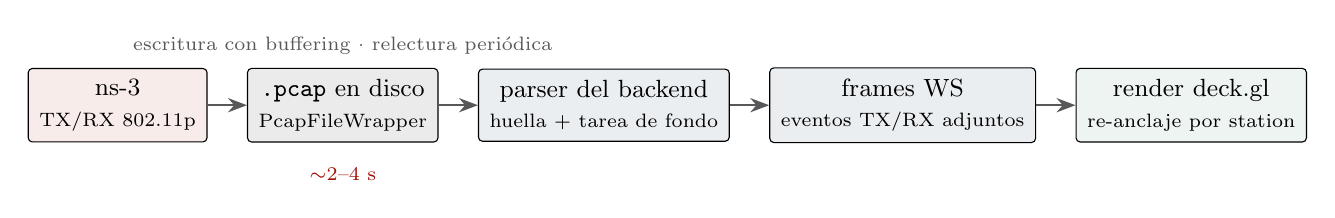
\begin{tikzpicture}[font=\small, node distance=4mm and 5mm,
  caja/.style={draw, rounded corners=1.5pt, align=center, minimum height=9mm, inner sep=4pt},
  fl/.style={-{Stealth[length=2.4mm]}, thick, color=gris}]
  \node[caja, fill=rojo!8]  (ns3)  {ns-3\\\scriptsize TX/RX 802.11p};
  \node[caja, fill=gris!12, right=of ns3]  (pcap) {\texttt{.pcap} en disco\\\scriptsize PcapFileWrapper};
  \node[caja, fill=azul!8,  right=of pcap] (parse){parser del backend\\\scriptsize huella + tarea de fondo};
  \node[caja, fill=azul!8,  right=of parse](ws)   {frames WS\\\scriptsize eventos TX/RX adjuntos};
  \node[caja, fill=verde!8, right=of ws]   (rend) {render deck.gl\\\scriptsize re-anclaje por station};
  \draw[fl] (ns3) -- (pcap);
  \draw[fl] (pcap) -- (parse);
  \node[above=0.5mm of pcap, color=gris] {\scriptsize escritura con buffering · relectura periódica};
  \draw[fl] (parse) -- (ws);
  \draw[fl] (ws) -- (rend);
  \node[below=2mm of pcap, color=rojo] {\scriptsize $\sim$2--4 s};
\end{tikzpicture}
\caption{Cadena captura\,$\to$\,disco\,$\to$\,parser\,$\to$\,WebSocket\,$\to$\,render.
El eslabón lento es el primero: ns-3 escribe los pcap con \emph{buffering}, así
que los arcos aparecen en el visor unos segundos después de la transmisión
real. Es un retardo honesto del pipeline, no un error.}
\label{fig:cadena}
\end{figure}

Dos decisiones de ingeniería sostienen esta cadena sin congelar el visor:
el índice V2X se reconstruye en una \textbf{tarea de fondo} (nunca en el
camino caliente del bucle de frames --- ver el caso de depuración 5), y el
refresco se \emph{auto-regula}: se espera al menos
3$\times$ la duración del último parseo antes de volver a parsear, de modo que
un pcap cada vez más grande no acapare la CPU.

\subsection{Reutilizar software libre: patrones frente a código}
\label{sec:mit}

Varias de las funciones de esta práctica están inspiradas en
\texttt{gods-eye-view}, un visor geoespacial open source (licencia MIT) con
estética de ``satélite de vigilancia'' construido sobre CesiumJS. Integrarlo
directamente era inviable --- motor distinto (Cesium+Vite frente a
MapLibre+deck.gl sin paso de build) --- así que se portaron \emph{patrones},
no código:

\begin{center}\small
\begin{tabular}{@{}p{0.44\linewidth}p{0.48\linewidth}@{}}
\toprule
\textbf{Patrón en gods-eye-view} & \textbf{Adaptación en SUMO-GEO} \\
\midrule
Cámara \emph{cockpit} dentro de un avión & Cámara persecución de un vehículo SUMO \\
\emph{Reskin reality}: shaders CRT/NVG/FLIR & Filtros CSS sobre el mapa + \emph{scanlines} \\
Overlay de detección (cajas + IDs) & HUD: caja y etiqueta \texttt{veh<station>} \\
``Render one interval behind'' & Ventana de interpolación estirada (\S\ref{sec:interp}) \\
Iconos estables en pantalla & No aplicaba: nuestros vehículos ya son geometría 3D orientada por rumbo real \\
\bottomrule
\end{tabular}
\end{center}

\begin{notabox}[ de propiedad intelectual]
La licencia MIT permite estudiar, adaptar y redistribuir el \emph{código},
pero no cubre necesariamente los \emph{assets} (modelos 3D, imágenes, datos)
del proyecto, que pueden tener licencias propias. Portar ideas y patrones de
diseño --- como aquí --- es siempre legítimo; copiar código exige respetar la
licencia (atribución en MIT); copiar assets exige revisar su licencia una a
una.
\end{notabox}

% ============================================================================
\section{Requisitos previos}
% ============================================================================

\begin{enumerate}[leftmargin=1.6em, itemsep=2pt]
  \item Práctica de instalación completada: stack \texttt{van3twin} operativo.
  \item Práctica de Replay completada (teoría y flujo de pcaps ya conocidos).
  \item El backend actualizado incluye el modo vivo y el control de velocidad
        del replay. Tras un \texttt{git pull} de \texttt{SUMO\_GEO}, reconstruir
        \textbf{una vez}:
\end{enumerate}

\begin{enmac}
\begin{lstlisting}
cd ~/van3twin-docker
docker compose --profile visor build backend
docker compose --profile visor up -d
\end{lstlisting}
Recordatorio: nunca \texttt{docker compose build} a secas (reconstruiría
también la imagen grande de ns-3). El frontend no necesita build: nginx sirve
los estáticos con \texttt{no-store}; basta recargar el navegador.
\end{enmac}

% ============================================================================
\section{Parte 1 --- Mensajes V2X en vivo}
% ============================================================================

Hasta ahora el visor en vivo mostraba \emph{solo} la movilidad; los mensajes
exigían esperar al replay. Ya no: el backend relee en caliente los pcap que
ns-3 escribe en su directorio de trabajo (el volumen ya está montado en
\texttt{/ns3}; la ruta la fija \texttt{APP\_LIVE\_PCAP\_DIR=/ns3/ns-3-dev}) y
adjunta los eventos TX/RX a los frames en vivo.

\begin{encontenedor}
\begin{lstlisting}
cd ~/VaN3Twin/ns-3-dev
./ns3 run "v2v-emergencyVehicleAlert-80211p --sumo-gui=false
           --met-sup=true --sim-time=300 --num-traci-clients=2"
\end{lstlisting}
SUMO queda ``waiting for 2 clients''; el visor lo destraba al conectarse.
\end{encontenedor}

\begin{ennavegador}
Abrir \url{http://localhost:8081}. A los pocos segundos de arrancar la
corrida:
\begin{itemize}[leftmargin=1.4em, itemsep=1pt]
  \item Brotan \textbf{pulsos} (transmisiones) y \textbf{arcos} (recepciones)
        sobre los vehículos en movimiento.
  \item El panel \emph{Replay V2X} revela automáticamente ``Mensajes V2X'',
        los filtros CAM/CPM/DENM y la fila \textbf{Emisor} (se puebla sola con
        las estaciones que van apareciendo; al elegir una, anillo ámbar sobre
        el emisor y solo sus mensajes en pantalla).
  \item El \textbf{panel PHY} muestra las estadísticas \emph{de la corrida en
        curso} y se refresca cada 10 s: latencia, cobertura, PER y utilización
        van creciendo con la corrida.
\end{itemize}
Las etiquetas de los arcos muestran \textbf{metros} (distancia entre las
posiciones TraCI en vivo de emisor y receptor) y \textbf{dBm} si el EVA
parcheado está volcando \texttt{signal-rx.csv} en el mismo directorio.
\end{ennavegador}

\begin{notabox}[: el retardo es real]
Los arcos aparecen $\sim$2--4 s después de la transmisión: es el buffering de
escritura de ns-3 más el ciclo de relectura (figura~\ref{fig:cadena}). La
movilidad, en cambio, llega por TraCI sin pasar por disco: por eso los
vehículos se mueven ``al día'' y los mensajes van unos segundos por detrás.
Distinguir ambos caminos es parte del ejercicio~\ref{ej:retardo}.
\end{notabox}

% ============================================================================
\section{Parte 2 --- Cámara cockpit (seguir a un vehículo)}
% ============================================================================

\begin{ennavegador}
\begin{enumerate}[leftmargin=1.6em, itemsep=1pt]
  \item Clic \textbf{derecho} sobre cualquier vehículo $\to$ en el popup,
        botón \emph{``Seguir este vehículo''}.
  \item La cámara se coloca en persecución: inclinación 76$^{\circ}$, zoom
        19.3, orientada al rumbo del vehículo. Un \emph{badge} flotante
        muestra en vivo id, rumbo y km/h.
  \item Salir: botón de cierre del badge, arrastrar el mapa o usar el pad.
\end{enumerate}
Combinación útil: seguir a la \textbf{ambulancia} del escenario EVA con el
filtro Emisor puesto en su station --- se ve el DENM de emergencia saliendo
del propio vehículo que la cámara persigue.
\end{ennavegador}

% ============================================================================
\section{Parte 3 --- HUD de detección y filtro Emisor}
% ============================================================================

El checkbox \emph{Detección} del panel principal activa un HUD estilo sistema
de percepción: caja verde y etiqueta \texttt{veh<station>} sobre cada
vehículo. Sirve para responder de un vistazo ``¿qué está viendo/etiquetando la
plataforma?'' y para cruzar el station del HUD con el filtro Emisor y con los
receptores listados en el popup de un mensaje.

\begin{notabox}
El HUD comparte el límite de nivel de detalle del visor
(\texttt{LOD\_MAX\_DETAILED}): con flotas muy grandes las cajas se apagan
automáticamente, igual que el detalle 3D de los vehículos.
\end{notabox}

% ============================================================================
\section{Parte 4 --- Modos sensor}
% ============================================================================

El selector de la barra superior cicla la ``óptica'' del visor:
\textbf{Normal / NVG} (visión nocturna) \textbf{/ FLIR} (térmica)
\textbf{/ Noir / CRT} (monitor antiguo con \emph{scanlines} y viñeta).
Técnicamente son filtros CSS aplicados al elemento del mapa --- mapa y overlay
deck.gl comparten elemento, así que vehículos y mensajes heredan el mismo
tratamiento. Útiles para presentaciones y para las capturas de los informes.

% ============================================================================
\section{Parte 5 --- Replay mejorado}
% ============================================================================

Con la corrida terminada, publicar los resultados y entrar en replay:

\begin{encontenedor}
\begin{lstlisting}
cp v2v-EVA-*.pcap signal-rx.csv ~/results/
\end{lstlisting}
No hace falta reiniciar nada: el backend detecta los ficheros nuevos solo.
\end{encontenedor}

\begin{ennavegador}
Novedades respecto a la práctica anterior:
\begin{itemize}[leftmargin=1.4em, itemsep=1pt]
  \item \textbf{Barra de tiempo} estilo reproductor: progreso relleno y
        tiempos \texttt{m:ss} actual/total.
  \item \textbf{Velocidad} (fila tortuga--liebre): 0{,}25$\times$ a 4$\times$
        sobre \emph{tiempo real}. A 1$\times$ un segundo de pared es un segundo
        simulado, con granularidad de 0{,}1 s por frame $=$ un CAM a 10 Hz
        (\S\ref{sec:relojes}).
  \item \textbf{El pulso de transmisión ES la cobertura}: el anillo se expande
        exactamente hasta el percentil 95 del alcance medido en la corrida (el
        valor \emph{Cobertura p95} del panel PHY).
  \item Persistencia por tipo de evento: los arcos RX viven 2{,}6 s (tiempo de
        sobra para clicarlos e inspeccionar el ASN.1); los pulsos TX, 1{,}2 s.
  \item Pulsos y arcos van \emph{anclados} a los vehículos dibujados: nacen y
        viajan con la posición interpolada, sin adelantarse.
\end{itemize}
\end{ennavegador}

% ============================================================================
\section{Casos reales de depuración}
% ============================================================================

Estas seis fallas aparecieron (y se corrigieron) durante el desarrollo de lo
que acabas de usar. Cada una ilustra un concepto general; ninguna se veía en
el código a simple vista. Léelas como mini-casos: síntoma $\to$ causa $\to$
arreglo $\to$ concepto.

\begin{casobox}[1: el vehículo que avanza y se para]
\textbf{Síntoma:} movimiento a tirones pese a la interpolación.
\textbf{Causa:} la ventana de interpolación usaba la \emph{media} del período
entre frames; con jitter, la mitad de los frames llegan más tarde que la media
y el vehículo espera parado. \textbf{Arreglo:} ventana estirada 30\,\%
(\texttt{INTERP\_STRETCH}); cada frame reinicia desde la posición \emph{ya
dibujada}, así el error se autocorrige sin saltos. \textbf{Concepto:}
interpolación con retardo vs.\ extrapolación; jitter buffers
(\S\ref{sec:interp}).
\end{casobox}

\begin{casobox}[2: el replay que iba a 5$\times$]
\textbf{Síntoma:} el replay ``corría'' aunque nadie tocó nada; en vivo no
pasaba. \textbf{Causa:} 10 fps $\times$ 0{,}5 s/frame $=$ 5 s simulados por
segundo. En vivo no se nota porque ns-3, en lockstep, marca el ritmo.
\textbf{Arreglo:} desacoplar render (10 fps fijos) de avance simulado (el
comando \texttt{speed} del WebSocket acepta ahora el paso por frame).
\textbf{Concepto:} los tres relojes de \S\ref{sec:relojes}.
\end{casobox}

\begin{casobox}[3: ``Seguir vehículo'' se autocancelaba]
\textbf{Síntoma:} la cámara persecución moría al instante de activarla.
\textbf{Causa:} mover la cámara por código (\texttt{map.jumpTo}) dispara el
mismo evento \texttt{rotatestart} que un gesto del usuario; el manejador
``cancelar si el usuario rota'' mataba el seguimiento en el primer frame de la
propia cámara. \textbf{Arreglo:} distinguir gesto real de evento programático
(guard \texttt{e.originalEvent}). \textbf{Concepto:} los sistemas de eventos
no distinguen por defecto quién originó el evento; hay que preguntarlo.
\end{casobox}

\begin{casobox}[4: el botón inclickeable]
\textbf{Síntoma:} un botón dentro del popup ignoraba los clics.
\textbf{Causa:} heredaba \texttt{pointer-events:none} del popup no
interactivo. \textbf{Arreglo:} \texttt{pointer-events:auto} en el elemento.
\textbf{Concepto:} las propiedades CSS heredadas o en cascada afectan a hijos
que ``no se ven'' afectados; depurar con el inspector, no con el ojo.
\end{casobox}

\begin{casobox}[5: pausas periódicas en vivo]\label{caso:pausas}
\textbf{Síntoma:} el stream en vivo se congelaba $\sim$0{,}5 s cada $\sim$2 s.
\textbf{Causa:} el bucle de frames hacía \texttt{await} del re-parseo del
índice V2X; como el pcap \emph{crece continuamente}, la huella cambiaba en
cada chequeo y el parseo (CPU-bound) bloqueaba el envío de frames.
\textbf{Arreglo:} caché sin bloqueo + reconstrucción en tarea de fondo con
throttle adaptativo (3$\times$ la duración real del último parseo).
\textbf{Concepto:} en un event loop (asyncio) nunca se bloquea el camino
caliente; el trabajo pesado va a hilos o tareas de fondo.
\end{casobox}

\begin{casobox}[6: arcos adelantados a sus vehículos]
\textbf{Síntoma:} los arcos nacían ``delante'' del vehículo que los emitía.
\textbf{Causa:} los arcos usaban la posición \emph{cruda} del último frame; los
vehículos dibujados van $\sim$medio período por detrás (interpolación con
retardo). Dos fuentes de verdad para la misma posición. \textbf{Arreglo:}
re-anclar pulsos y arcos por station a la posición \emph{interpolada} en cada
tick de render. \textbf{Concepto:} cuando dos capas visualizan el mismo objeto,
deben compartir la misma fuente de posición.
\end{casobox}

% ============================================================================
\section{Ejercicios}
% ============================================================================

\begin{tareabox}
\begin{enumerate}[leftmargin=1.6em, itemsep=4pt]
  \item \textbf{¿Quién marca el reloj?} Reproduce la MISMA corrida en vivo y
        en replay. ¿Por qué el replay admite 4$\times$ y el vivo no admite
        acelerarse? ¿Qué limitaría al vivo si quisiéramos acelerarlo?
        Responde usando los tres relojes de \S\ref{sec:relojes}.
  \item \textbf{La ambulancia.} Con cockpit + filtro Emisor, sigue a la
        ambulancia del EVA. Anota qué tipos de mensaje emite, con qué
        frecuencia aparecen sus pulsos y qué vehículos aparecen como
        receptores en el popup cuando pasa cerca de ellos.
  \item \label{ej:retardo}\textbf{El retardo del vivo.} Cronometra cuánto
        tardan los arcos en aparecer tras arrancar la corrida. Explica el
        retardo eslabón por eslabón con la figura~\ref{fig:cadena}, y explica
        por qué la \emph{movilidad} no sufre ese retardo.
  \item \textbf{Cobertura visible.} En replay, mide a ojo (con las etiquetas
        de distancia de los arcos como regla) el radio final de un pulso TX y
        compáralo con el valor \emph{Cobertura p95} del panel PHY. ¿Por qué se
        eligió el p95 y no el máximo?
  \item \textbf{Path-loss otra vez.} Con las etiquetas ``m $\cdot$ dBm'' de al
        menos cinco arcos a distintas distancias, estima el exponente $n$ de
        log-distancia (método de la práctica de Replay) y compáralo con el
        modelo configurado en ns-3 (LogDistance, $n=3{,}0$).
  \item \textbf{Depuración guiada (opcional, para valientes).} En
        \texttt{app.js}, comenta el guard \texttt{e.originalEvent} del
        manejador de rotación y recarga. Activa ``Seguir vehículo'' y describe
        lo que ocurre y por qué (caso 3). Restaura el guard al terminar.
  \item \textbf{Granularidad.} A 1$\times$ el replay avanza 0{,}1 s simulados
        por frame. ¿Qué relación tiene ese número con la frecuencia de
        generación de CAM? ¿Qué se ``perdería'' visualmente con 0{,}5 s por
        frame?
\end{enumerate}
\end{tareabox}

% ============================================================================
\section{Entregables}
% ============================================================================

Informe breve (PDF) con: respuestas razonadas a los ejercicios 1--5 y 7
(el 6 es opcional), capturas del visor que respalden cada respuesta
(los modos sensor son bienvenidos para las capturas), y una reflexión final de
un párrafo: ¿qué aporta ver los mensajes \emph{en vivo} que no aporta el
replay, y viceversa?

\vspace{8pt}\hrule\vspace{6pt}
{\small\color{gris} Universidad de Cuenca · Redes Vehiculares y Heterogéneas ·
Prácticas del gemelo digital VaN3Twin + SUMO-GEO. Prerrequisitos:
\emph{Práctica de instalación del framework} y \emph{Práctica Replay V2X}.}

\end{document}
